\documentclass[border=10pt]{standalone}

\usepackage{tikz}
\usepackage{tikzsymbols}
\usetikzlibrary{calc,patterns,shapes.geometric}

\def\centerarc[#1](#2)(#3:#4:#5){\draw[#1] ($(#2)+({#5*cos(#3)},{#5*sin(#3)})$) arc (#3:#4:#5);}

\begin{document}
	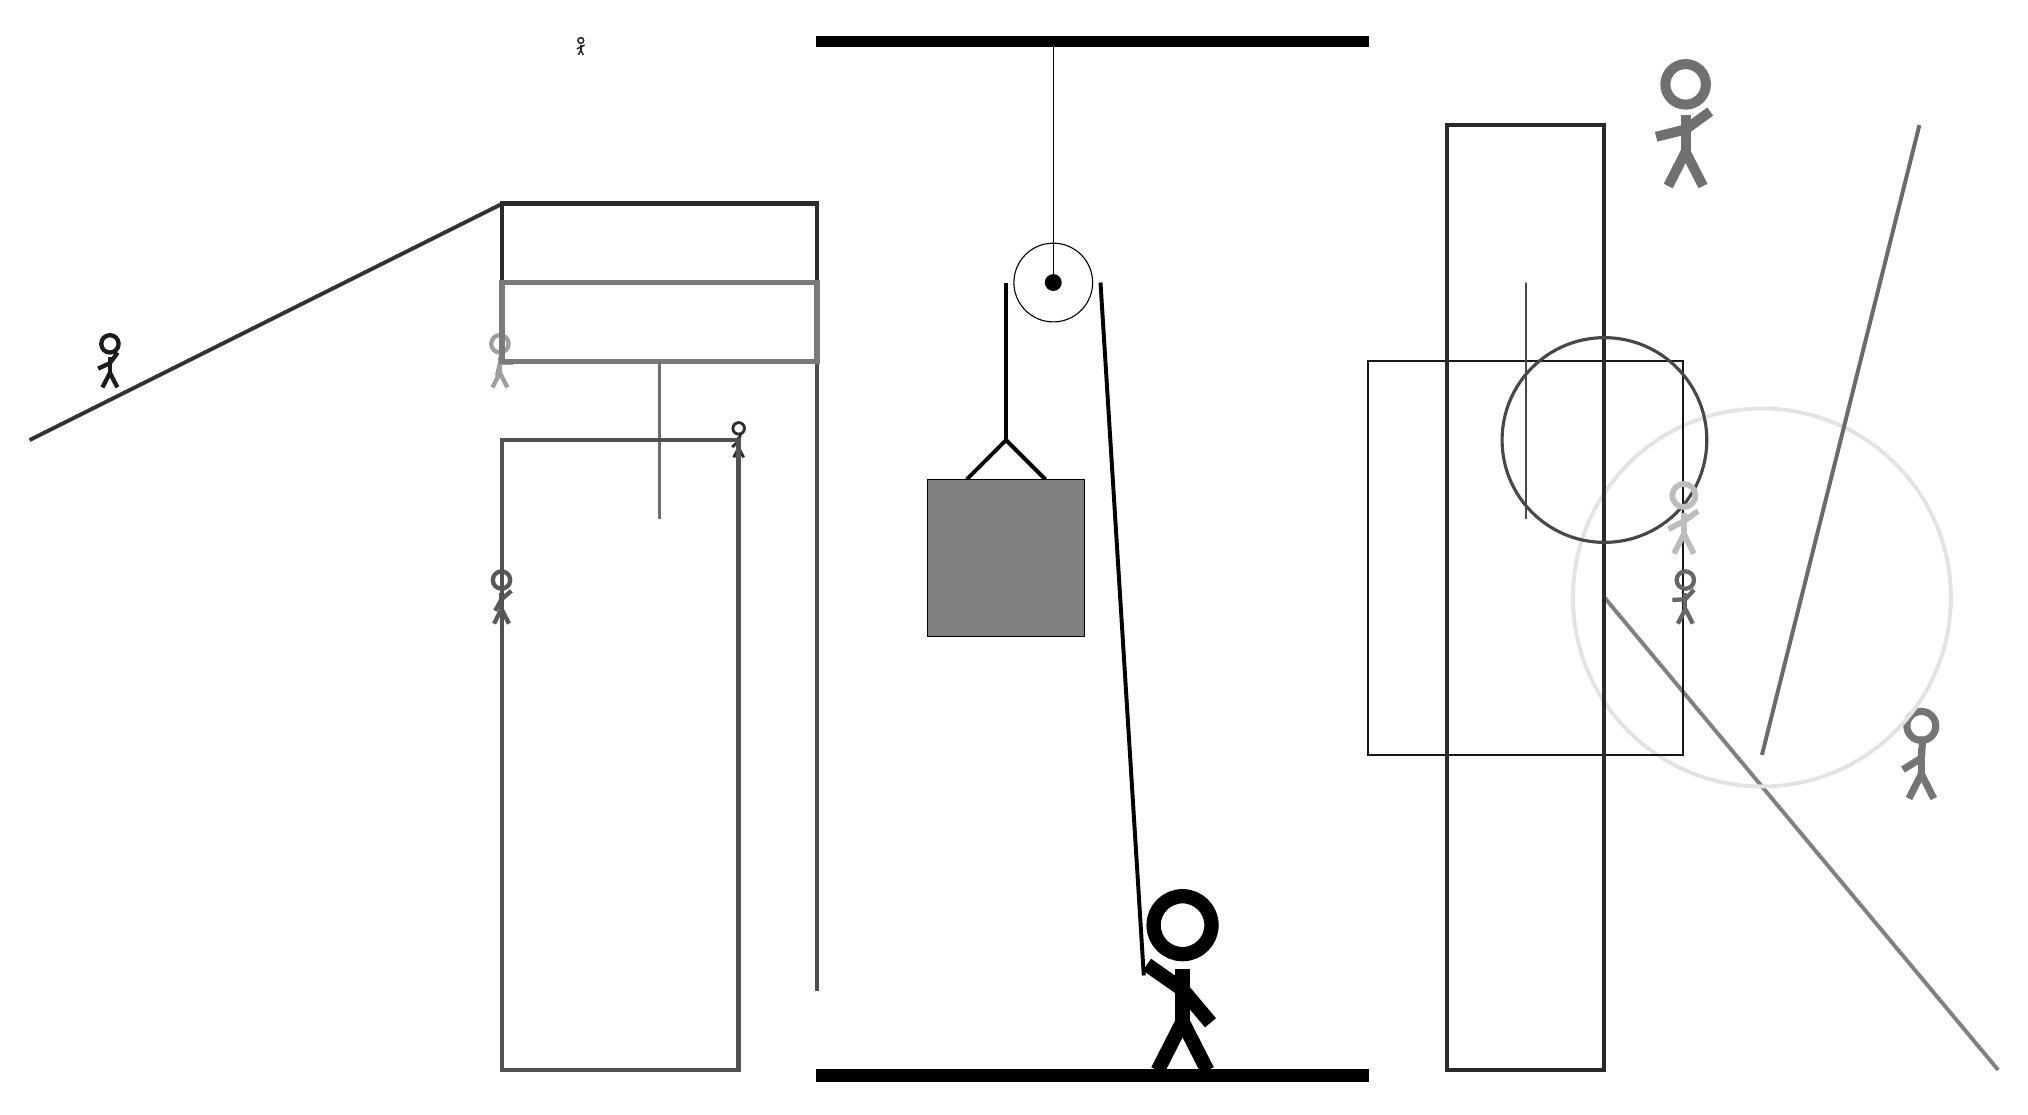
\begin{tikzpicture}
		%%%%% START %%%%%
		
		\draw[fill=black] (-2, 10) rectangle (5, 10.125);
		
		\draw (1, 7) circle (0.5);
		\draw[fill=black] (1, 7) circle (0.1);
		\draw (1, 10) -- (1, 7);
		
		\draw[line width=0.5mm] (-0.1, 4.5) -- (0.4, 5.0) -- (0.9, 4.5);
		\draw[fill=black!50] (-0.6, 4.5) rectangle (1.4, 2.5);
		
		\draw[line width=0.5mm, color=black!80](-6, 8) -- (-12, 5);
		
		\draw[line width=0.5mm, color=black!69](-2, -2) -- (-2, 8);
		\draw [line width=0.7mm, color=black!55](-5, 6) circle (0.0);
		\draw[line width=0.5mm, color=black!50](8, 3) -- (13, -3);
		
		\draw[line width=0.6mm, color=black!83] (-2, 6) rectangle (-6, 8);
		\node[line width=0.6mm, color=black!82] at (-3, 5) {\Strichmaxerl[2][41][76]};
		\node[line width=0.7mm, color=black!54] at (12, 1) {\Strichmaxerl[5][32][86]};
		\draw [line width=0.5mm, color=black!11](10, 3) circle (2.4);
		\node[line width=0.5mm, color=black!56] at (9, 9) {\Strichmaxerl[7][14][36]};
		\node[line width=0.7mm, color=black!65] at (-6, 3) {\Strichmaxerl[3][61][41]};
		\node[line width=0.4mm, color=black!38] at (-6, 6) {\Strichmaxerl[3][77][0]};
		\draw[line width=0.7mm, color=black!52] (-2, 7) rectangle (-6, 6);
		\node[line width=0.3mm, color=black!87] at (-5, 10) {\Strichmaxerl[1][27][27]};
		\draw[line width=0.3mm, color=black!91] (5, 6) rectangle (9, 1);
		\draw[line width=0.5mm, color=black!84] (6, 9) rectangle (8, -3);
		\draw[line width=0.4mm, color=black!57] (-4, 4) rectangle (-4, 6);
		
		\node[line width=0.7mm, color=black!60] at (9, 3) {\Strichmaxerl[3][2][48]};
		\node[line width=0.6mm, color=black!89] at (-11, 6) {\Strichmaxerl[3][25][54]};
		\draw [line width=0.4mm, color=black!72](8, 5) circle (1.3);
		
		\draw[line width=0.3mm, color=black!72] (7, 7) rectangle (7, 4);
		\node[line width=0.3mm, color=black!26] at (9, 4) {\Strichmaxerl[4][27][36]};
		
		\draw[line width=0.6mm, color=black!68] (-3, 5) rectangle (-6, -3);
		\draw[line width=0.5mm, color=black!58](10, 1) -- (12, 9);
		
		\draw[line width=0.5mm] (0.4, 7) -- (0.4, 5.0);
		\centerarc[line width=0.5mm](1, 7)(0:180:0.6);
		\draw[line width=0.5mm](1.6, 7) -- (2.15, -1.8);
		
		\node at (2.6, -1.9) {\Strichmaxerl[10][-35][-50]};
		
		\draw[fill=black] (-2, -3) rectangle (5, -3.15);
		
		%%%%% END %%%%%
	\end{tikzpicture}
\end{document}